 \setlength{\baselineskip}{20pt}
\chapter{引言}
\label{cha:intro}

\section{研究背景及意义}

随着城市化进程的持续推进，城市道路资源与停车资源之间的矛盾日益凸显。停车难、泊车效率低以及因泊车不当引发的交通安全问题，已成为制约城市交通运行效率和居民出行体验的关键因素~\cite{liqian2019}。在此背景下，自动泊车系统作为智能交通与自动驾驶技术的重要组成部分，正逐步从辅助功能向高可靠性的智能系统演进（如图 \ref{fig_intro} 所示）。停车位检测作为自动泊车系统中的核心感知环节，其性能直接决定了后续泊车路径规划与控制决策的准确性与安全性。

在自动泊车系统的感知方案中，传感器选择是影响系统性能与成本的关键因素。目前主流方案包括视觉、雷达、激光雷达等多种技术路线。其中，基于摄像头的视觉感知方案因其成本低、信息丰富和易于部署等优势，成为当前研究与工业界关注的焦点~\cite{yan2024}。相较于雷达等传感器，视觉方法能够提供更加精细的几何与语义信息，适用于复杂多样的停车场环境。然而，停车位检测任务本身具有目标结构复杂、尺度变化大以及场景干扰因素多等特点，使其在实际应用中面临诸多挑战。

\begin{figure}[!h] % use float package if you want it here
  \centering
  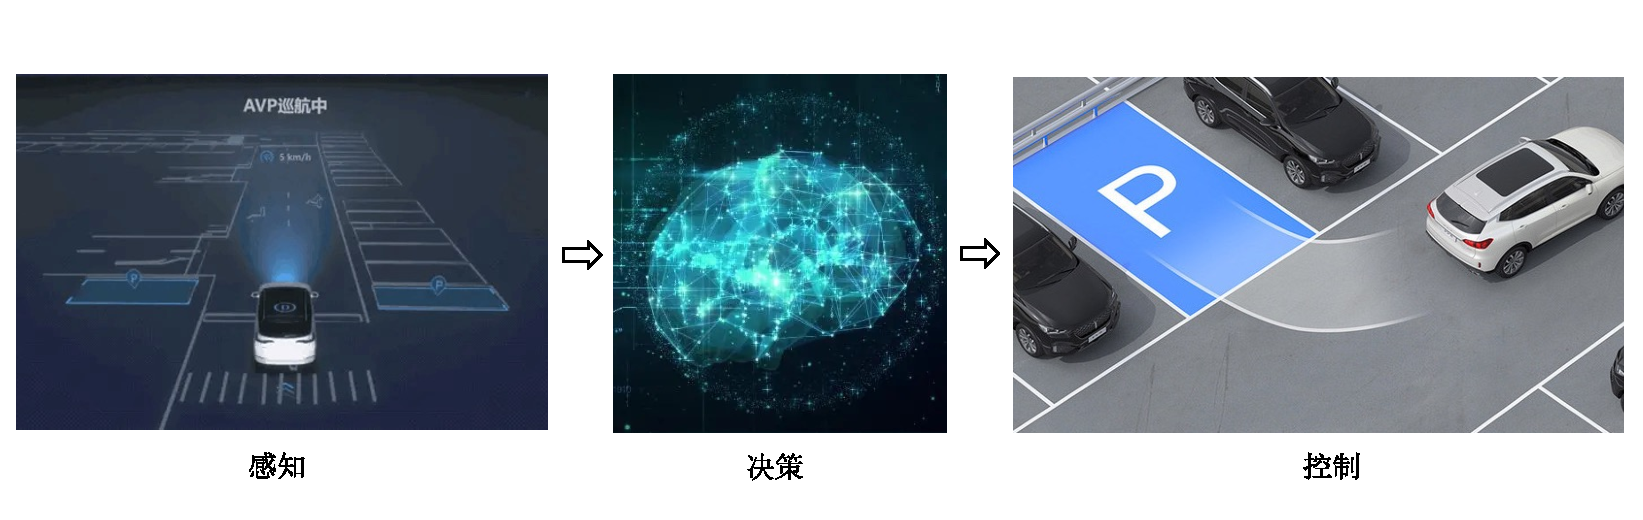
\includegraphics[width=1\linewidth]{figures/chp0/intro.pdf}
  \caption{智能泊车系统示意图  \\Figure~\ref{fig_intro} Architecture of the intelligent parking system}
  \label{fig_intro}
\end{figure}

从目标属性角度来看，停车位并非传统意义上的刚性目标，而是由多条标线和多个关键点共同构成的结构化目标。其几何形态在不同场景中呈现显著差异，例如垂直车位、平行车位和倾斜车位等形式，在关键点分布与结构关系上存在明显不同。此外，停车位通常呈现高密度分布特征，相邻车位之间结构相似，容易在视觉感知过程中产生混淆。这些因素使得停车位检测不仅需要准确的局部特征提取能力，还对模型的结构建模能力提出了更高要求。

从数据获取与模型训练的角度来看，高质量标注数据的获取成本始终是制约停车位检测研究的重要瓶颈。停车位的标注通常涉及多个关键点及其对应关系，标注过程复杂且耗时，难以在大规模、多场景条件下快速扩展。这导致现有公开数据集在规模、场景多样性以及极端复杂条件覆盖方面仍存在不足，进而限制了基于全监督学习方法在真实场景中的泛化能力。如何在有限标注数据条件下充分利用未标注数据，成为停车位检测研究中亟需解决的问题。

在方法设计层面，尽管近年来深度学习技术显著推动了停车位检测性能的提升，但部分现有方法仍沿用“检测 + 后处理”的传统流程，即先预测局部特征或关键点，再通过人工设计的规则对检测结果进行组合与匹配。这类方法在特定场景下能够取得较好效果，但其性能往往依赖于经验性规则与阈值设置，在复杂光照、局部遮挡或停车位密集等情况下容易出现结构不一致或匹配错误的问题。其中，缺乏在模型训练阶段对停车位结构关系的显式建模，是造成上述问题的重要原因之一。

此外，从实际应用场景来看，车辆在泊车过程中获取的是连续的多帧视觉信息，而非孤立的单帧图像。单帧检测方法在面对动态视角变化、短时遮挡以及环境噪声时，容易产生检测结果波动，从而影响系统整体的稳定性与可靠性。然而，现有研究中仍有相当一部分工作主要聚焦于单帧检测任务，未能充分挖掘时序信息在提升停车位检测稳定性方面的潜力。如何将空间结构建模与时间维度信息有机结合，构建更加鲁棒的停车位检测方法，是当前研究中的一项重要挑战。

综上所述，停车位检测在复杂真实场景下仍面临数据受限、结构建模不足以及时序信息利用不充分等问题，亟需从数据、方法建模以及时空融合等多个层面开展系统研究。针对这些问题，本文围绕复杂场景下的停车位检测任务，从数据与学习范式、空间结构感知建模以及多帧时序建模三个层面展开深入研究，具有重要的理论意义与实际应用价值。


\section{研究现状}
\subsection{基于传统算法的停车位检测方法}

（1）基于直线的方法

停车位是停车场内由引导线和分隔线围成的地面区域，主要包括矩形、平行四边形及菱形等多种类型。由于停车位标识由直线段构成，因此直线识别成为停车位检测的关键环节~\cite{ma2021research}。

针对这一关键环节，Jung等人\cite{jung20063d}提出了一种融合像素分类与特征匹配的方法，用于提取停车场的空间结构信息。该方法首先利用平面约束提取停车场标线并转换为俯视图，随后在俯视图基础上通过模板匹配精确定位车位。此外，研究者还利用相邻车辆的视差生成障碍物深度图，通过限定搜索范围与方向，将其作为模板匹配的判别准则。实验结果表明，该方法结合障碍物深度信息与标线俯视图，不仅有效缩小了算法的搜索空间，还显著提升了运算速度及对视觉噪声的鲁棒性。

然而，车载摄像头在光照剧变（如夜间或逆光环境）时的稳健性仍然是一个挑战。针对这一问题，Kamiyama等人\cite{kamiyama2019recognition}提出了一种全天候停车位识别方法，使其在昼夜更替或路面干湿变化的情况下均能正常工作。该方法利用激光测距仪获取接收光强值的统计模型，据此对路面进行分类，并结合霍夫变换（Hough Transform）估计目标停车位置。此外，Jung等人\cite{jung20063d}针对自动泊车辅助系统的车位自动选择问题，提出了一种基于单目视觉的车位线识别算法。该研究在霍夫空间中设计了一维滤波器，利用边缘图像俯视图中车位线特征的先验知识，并引入改进的点到线段距离测度来区分识别出的线段。实验结果表明，即便在相邻车辆严重遮挡车位线的情况下，该算法仍能成功识别车位。

霍夫变换常被用于检测车位标线，但受噪声、杂乱背景、光照波动及天气变化等因素干扰，其在检测平行线对时的稳健性较差，且无法同时检测多个平行线对。针对上述缺陷，Wang等人\cite{wang2014automatic}采用多项式鱼眼畸变模型对摄像头进行标定，并利用基于 Levenberg-Marquardt 算法的图像拼接技术，将四个鱼眼摄像头的图像合成为全向俯视图。在此基础上，该研究引入了基于拉东变换（Radon Transform）的车位特征提取方法，实现了对多个车位的同步检测。此外，文中还指出了其他传感方案的局限性：当超声波传感器的探测距离小于3米时，其测量结果无法为障碍物识别提供有效信息；同时，仅基于后视摄像头的系统由于视野受限，在平行泊车等需要宽阔视野的场景中难以发挥辅助作用。

为了获得更宽阔的视野，研究人员开始探索全景视觉技术在车位检测中的应用。Hamada等人\cite{hamada2015surround}提出了一种基于全景图像的车位检测算法，有效解决了目标车位移出当前视场时的跟踪丢失问题。为提升检测精度，Lee等人\cite{lee2016available}设计了一种锥形帽标线提取滤波器及基于熵的标线聚类算法；即便在能见度较低的情况下，该滤波器仍能强力提取线条特征，随后由聚类算法高效地将特征分配至各车位线段。与霍夫变换等传统线性检测器相比，该方法在处理畸变或模糊标线时速度更快、稳健性更强，且在目标位置与偏航角估计的准确度上优于基于角点检测的方法。

然而，现有方法在处理复杂障碍物干扰和识别微小障碍物方面仍存在不足。针对这些问题，Li等人\cite{li2017automatic}提出了一种基于环视系统（Around View Monitor，AVM）的自动检测方案。该方案利用直线段检测器（Line Segment Detector，LSD\cite{von2012lsd}）在全景图像中识别固定间距的平行标线，并结合图像分割与立体视觉算法计算标线高度，从而识别车位内的细小障碍。实验结果证明，该方法在检测的连续性与完整性上优于霍夫变换，显著降低了误报率与漏检率。在此基础上，Wenhao等人\cite{zong2018robust}对 LSD 算法进行了改进，将其划分为检测与跟踪双线程：检测线程利用改进的提取器获取线段边缘及L型组件结构信息，并结合前后帧关联搜索候选区域；跟踪线程则利用卡尔曼滤波（Kalman Filter）实时更新车位位置并给出置信度评分，最后辅以超声波验证以剔除伪目标。此外，Li等人\cite{li2018geometric}提出的基于几何特征的方法，通过线聚类与几何约束配对，在弱光、强光以及地砖、曲线等复杂路面条件下均表现出优异的全自动检测性能。

为了进一步提升车位检测的自动化程度和稳健性，Jae等人\cite{suhr2018universal}开发了一套全自动化的车位检测与识别方法，该方法能识别多种类型的车位标线，且在不同光照条件下展现出较强的稳健性。首先，该方法从环视系统图像中提取平行线对，以识别车位标线的分割线。随后，将当前帧检测到的分割线与前一帧结果进行融合，并依据车位几何约束对分割线进行配对，从而生成候选车位区域。在此基础上，系统利用直线与角点特征识别车位入口，并配合超声波传感器判断车位占用状态，以对候选车位进行验证。最后，系统将当前帧识别的空闲车位与历史帧结果进行合并，并基于车载运动传感器的里程计数据，实现对历史帧分割线及当前车位位置的持续跟踪。


（2）基于角点的方法

传统的基于直线检测的车位识别方法往往仅能识别一两种特定类型的车位，难以应对现实中如菱形或平行四边形等多样化的车位布局。相比之下，基于角点特征的检测方法能够识别多种车位类型，进而支持更复杂的泊车操作。Suhr等人\cite{suhr2013full}设计了一种全自动车位识别方案，该方案的核心在于将不同类型的车位标线建模为分层树状结构进行识别。该方法主要由“自底向上”与“自顶向下”两个过程组成：首先，通过自底向上的过程逐步生成候选车位；随后，根据车位标线类型的固有属性，沿树状结构自顶向下进行遍历，以剔除虚假车位、冗余节点及干扰角点。最终，系统确定目标车位的准确位置。尽管该方法实现了全自动化，但其在计算量保持较低水平的前提下，性能表现仍显著优于早期的半自动化方法。

在上述研究的基础上，Suhr等人\cite{suhr2013sensor}进一步提出了一套高效的车位检测与跟踪系统，该系统由三个核心阶段组成：在车位标线检测阶段，该研究沿用了文献\cite{suhr2013full}中的分层树状结构方法，实现了对多种车位类型的有效识别。在车位占用分类阶段，系统利用超声波传感器数据判定所检车位的空闲状态。该方法将每个车位区域视为独立的占用栅格单元，并据此计算占用概率。最后，在车位标线跟踪阶段，当车辆驶入车位时，系统会持续估计所选车位的位置。在跟踪过程中，系统在匹配得分层面融合了环视图像与基于运动传感器的测距信息，从而有效应对了车辆入库过程中不可避免的遮挡问题。实验结果表明，该系统能够实时识别各类车位的位置及占用情况，并在实际工况下实现稳定跟踪，既能辅助驾驶员快速选择可用车位，也能通过持续更新目标位置为泊车控制系统提供支持。

传统基于几何特征的方法虽然在特定场景下表现良好，但在处理复杂环境（如严重遮挡、光照变化剧烈等）时仍存在局限性。随着深度学习技术的快速发展，研究人员开始将深度学习算法应用于车位检测任务，以提高检测的鲁棒性和准确性。

\subsection{基于深度学习算法的停车位检测方法}
针对自动车位检测问题，已有大量研究聚焦于环视图像的应用，并由此催生出多种基于深度学习的检测方法。这些方法充分利用了环视图在空间覆盖上的全面性，旨在复杂多变的泊车环境中显著提升检测算法的准确度与稳健性~\cite{aajal2025autonomous}。

（1）基于目标检测的方法

Lin和Huang\cite{zhang2018vision}首次提出了深度停车位检测（DeepPS）方法，该方法基于深度学习，利用深层卷积神经网络（Deep Convolutional Neural Network，DCNN）来检测停车位。该方法对环视图像进行处理，采用两阶段检测流水线来定位和分类停车位特征。在第一阶段，该方法使用预先训练的基于 YOLOv2 的目标检测器识别输入图像中的所有标记点。在第二阶段，使用定制的 DCNN 分析检测到的标记点对，以确定它们是否形成有效的入口线，并将停车位类型分类为垂直、平行或倾斜。根据检测到的标记点和分类输出的空间形状，该方法可以对每个停车位的最终位置和方向进行几何估计。

为了进一步提升车位检测的精度和鲁棒性，Junhao和Zhang\cite{huang2019dmpr}提出了另一种值得注意的方法，名为方向标记点回归（DMPR-PS）。如图 \ref{fig_dmpr} 所示，该算法首先将输入图像送入卷积神经网络（Convolutional Neural Network，CNN）生成特征图；随后，利用这些特征图对定向标线点进行回归，这些点代表了候选车位的角点及其方向信息。接着，车位推断模块对标线点进行配对与筛选，从而锁定最终的车位位置。该方法采用多属性CNN回归模型估计车位的关键特征，包括标线点坐标、车位形状（如T型或L型）、朝向以及检测置信度。最终的车位识别通过一套过滤机制完成，该机制旨在剔除无效的标线点对。例如，同一车位内的两个标线点必须满足预设的最小空间距离阈值，且若两点连线被第三个中间点穿过，则该点对将被视为无效。最后，通过对验证后的定向标线点进行几何配对，形成入口线模式，从而实现对每个独立停车位的精准定位。


\begin{figure}[!h] % use float package if you want it here
%\setlength{\abovecaptionskip}{-0.2cm} %调整图片caption与正文之间的间距，table同理。可自己调整。
  \centering
  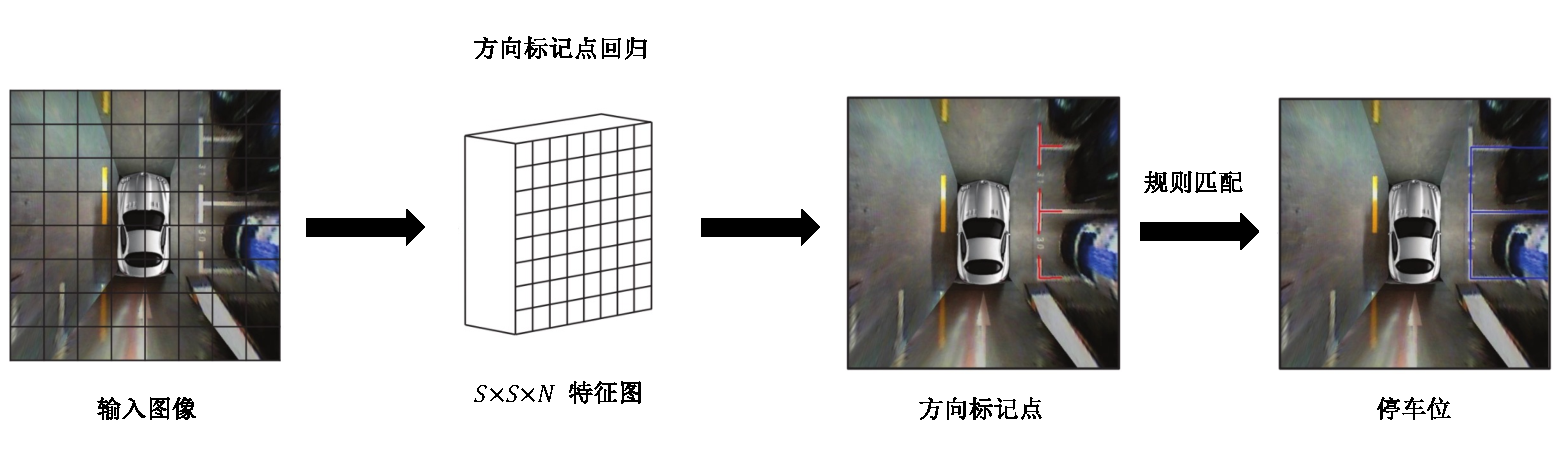
\includegraphics[width=1\linewidth]{figures/chp0/dmpr.pdf}
  \caption{DMPR-PS\cite{huang2019dmpr}算法流程图 \\Figure~\ref{fig_dmpr}~Pipeline of the DMPR-PS\cite{huang2019dmpr}}
  \label{fig_dmpr}
\end{figure}

在车位检测与占用状态识别的结合方面，Li等人\cite{li2020vacant}提出的空闲车位检测网络（VPS-Net）是另一种重要的研究方法。该方法基于YOLOv3\cite{redmon2018yolov3}目标检测模型，通过边界框（Bounding Boxes）对图像中的标线点与车位头进行定位与识别。随后，该系统通过分析成对标线点之间的几何距离以及所识别车位头的构型，推断出车位的具体类型；并进一步应用几何规则推算隐藏角点，从而将检测到的特征关联为完整的车位结构。在车位占用状态的判定上，VPS-Net 引入了基于 AlexNet~\cite{krizhevsky2012imagenet} 架构定制的深度卷积神经网络。与采用单一 CNN 进行检测的 DMPR-PS 不同，VPS-Net 采用了两阶段流水线：第一阶段利用 YOLOv3 检测车位头与标线点，第二阶段则独立对每个检测到的车位进行占用状态分类。

在上述研究的基础上，Wu等人\cite{wu2020psdet}提出的PSDet是一种更为通用且高效的解决方案。该方案采用两阶段级联神经网络架构，并引入了创新的圆形描述符（Circular Descriptor）框架。在第一阶段，该算法从环视输入图像剪裁出的左右子图中提取多尺度特征，随后通过 Softmax 归一化的响应图生成粗略的标线点候选区域。在第二阶段，使用基于 CNN 的精细回归模型对以这些候选区域为中心的小尺寸子图进行处理。在此过程中，圆形描述符被用于估计顶点的精确位置（以偏移量的形式表示）。由于圆形设计本质上具有旋转不变性，该模型能够稳健地应对各类复杂泊车场景中的方向变化。

考虑到模型的训练与推理效率，Li等人\cite{li2020parking}提出了一种深度卷积神经网络架构。该架构引入了定向入口线检测器，旨在估算车位入口线的中点，随后依据预定义的几何规则重构完整的车位几何形状。该定向入口线检测器由30个卷积层组成，并借鉴了 ResNet~\cite{kaiming2016deep} 的设计思路，集成了残差连接。这些残差连接有助于提升梯度流动的效率，从而增强模型的收敛性与训练稳定性。该网络通过预测入口线中点 $P(x,y)$，并根据车位入口的朝向将车位划分为直角、钝角或锐角三类。最后，该系统利用预测的中点坐标与分类结果，通过几何规则推算出车位的最终坐标，实现了对完整停车空间的快速且精准重建。

为了进一步简化检测流程并提高端到端性能，Suhr与Jung\cite{suhr2021end}提出了一种直接作用于环视系统图像的端到端车位检测方法。与早期依赖于节点配对和形状估计等人工几何启发式规则的方法不同，该方法利用卷积神经网络同时提取全局与局部特征。这种集成策略实现了对车位位置、类型、占用状态及节点方向的联合预测，无需复杂的基于规则的后处理过程。该算法首先将输入的AVM图像划分为网格，并利用 CNN 骨干网络（如去掉全连接层的VGG16）提取特征。以$416\times416$的输入尺寸为例，网络生成$13\times13\times512$的特征图，并进一步导出两个独立的输出张量：一个$13\times13\times9$的张量用于表征全局特征（涵盖车位入口、类型及占用情况），另一个$13\times13\times5$的张量用于表征局部特征（捕捉节点的精确位置与朝向）。在此基础上，Bui和Suhr\cite{bui2023cnn}提出了一种专门的两级停车位检测框架，证明了设计良好的两级结构在一般目标检测研究中的性能优于一级模型。在第一阶段，使用区域提案网络（Region Proposal Network，RPN）生成以入口中心、长度和方向为特征的区域提案来检测潜在的停车位入口。在第二阶段，该框架对提案进行细化，以产生停车位属性的精确估计，包括位置、类型和占有率。

Zinelli等人\cite{zinelli2019deep}提出了一种用于环视图像车位检测与占用分类的端到端深度神经网络。该方法基于改进的 Faster R-CNN 架构，并针对泊车环境中常见的几何多变性及斜向视角问题进行了优化。与传统目标检测方法回归轴对齐边界框不同，该模型能够预测通用的四边形框，从而对车位形状进行更灵活、更精确的表征。该架构实现了在各种复杂工况（包括多样的车位形状与朝向）下的稳健检测与分类。由于该模型具备同步进行定位与占用状态评估的能力，使其特别适用于复杂且真实的泊车环境部署。

基于目标检测的方法虽然在检测精度和鲁棒性方面有显著提升，但其依赖大量标注数据进行训练，标注成本较高。这类方法的后处理步骤往往较为复杂，仍需人工设计的几何规则。

% 除了基于目标检测的方法外，图像分割技术也在车位检测中得到了广泛应用，为识别车位标线提供了更精细的像素级信息。

（2）基于图像分割的方法

基于深度学习的车位检测方法广泛利用图像分割技术来识别并定位关键视觉特征。其中，语义分割（Semantic Segmentation）技术常用于对图像中的每个像素进行分类，从而有效区分车位标线与背景，并提供关于标线位置与形状的详细信息。与之不同，实例分割（Instance Segmentation）方法，尤其是基于 Mask R-CNN~\cite{he2017mask} 架构的方案，则侧重于检测并生成特定标线点（如T型或L型节点）的精确掩码，进而界定车位边界。

Jiang等人\cite{jiang2020detection}提出了一种集成深度学习与经典计算机视觉技术的车位检测方法。该方法采用以 ResNet-101 和特征金字塔网络（Feature Pyramid Network，FPN）为骨干网络的 Mask R-CNN 模型，通过生成实例分割掩码来检测T型和L型等交叉节点。在预处理阶段，该系统通过感兴趣区域选择与对比度增强提升图像质量；在检测完成后，该系统利用形态学操作对掩码进行细化，并结合 LSD 算法提取结构线与引导线。最终，该系统依据标线点分类结果与几何先验推断出车位的朝向与深度。尽管该方法在精度上有所提升，但其对 LSD 算法的依赖导致在直线检测效率方面存在不足。

为了提高环视图像的分割精度并减少对传统算法的依赖，Wu等人\cite{wu2018vh}提出了一种 VH-HFCN 网络，专门用于检测全景环视图像中的车位与车道线。该网络架构基于高度融合卷积网络（Highly Fused Convolutional Network，HFCN），并在上采样阶段前引入了“VH阶段”：该阶段由两个并行的卷积分支组成，分别采用垂直（$9\times1$）和水平（$1\times9$）卷积核。这一设计显著增强了网络对线性特征的提取能力。在分割任务完成后，该算法通过三个步骤进行后处理：首先，利用形态学骨架化提取中心线；然后，应用霍夫变换进行直线检测；最后，利用基于相似性的合并算法重构完整的车位几何形状。

与依赖几何模型的方案不同，Jang与Sunwoo\cite{jang2019semantic}提出了一种统一的感知系统，该系统能够在不依赖人工设计特征的前提下，同步检测车位标线与静态障碍物。该框架主要包含两个阶段：a. 语义分割阶段：采用具备编码器-解码器（Encoder-Decoder）结构的全卷积网络，将环视图像中的每个像素划分为四类：空闲空间、车位标线、车辆以及其他静态物体（如墙壁、路缘、柱子等）。b. 基于垂直栅格的检测阶段：对分割结果进行二值化、垂直编码、聚类及精细化处理。具体而言，该系统利用最优阈值对特定类别的分割图进行二值化，并采用垂直栅格编码技术将数据抽象为水平向量。随后，该系统通过对空单元格进行聚类以识别候选车位，最后通过精细化步骤估计每个车位的位置与朝向。这种基于栅格的后处理方式实现了高效且结构化的车位检测，无需传统的直线拟合或人工定义的启发式规则，使其非常适用于自动泊车系统的实时应用场景。

基于图像分割的方法虽然能够提供精细的像素级信息，但其计算复杂度较高，实时性表现较差。这类方法对标注数据的质量要求更高，后处理步骤也较为复杂，需要额外的几何约束，在低对比度或模糊场景下分割精度容易下降。

（3）基于结构化建模的方法

现有的许多用于停车位检测的深度学习方法依赖于复杂的后处理步骤，这既耗时又容易导致结果不准确。为解决这些问题，Min等人\cite{min2021attentional}提出了一种基于注意图神经网络（Attention-based Graph Neural Network，AGNN~\cite{thekumparampil2018attention}）的端到端可训练方法，消除了人工设计的后处理步骤。他们方法的核心思想是将环视图像中的标记点（即停车位的角点）表示为图结构的数据集。该模型利用图神经网络（Graph Neural Network，GNN\cite{scarselli2008graph}）对相邻标记点的上下文信息进行聚合，通过关系推理实现更准确的车位检测。该框架由三个主要模块组成：a. 图形特征编码器：AGNN 从环视图像中提取深层特征，以检测标记点位置并生成特征描述符。位置信息通过多层感知器（Multilayer Perceptron，MLP）嵌入，并与外观特征融合。b. 图特征聚合：构造一个全连通图，每个节点对应一个检测到的标记点。基于注意力的多头 GNN 聚集相邻节点的特征，捕捉几何和上下文依赖关系。c. 入口线鉴别器：对于一对标记点，它们的融合特征被串联并通过基于MLP的鉴别器，该鉴别器预测该对是否构成停车位的有效入口线。该方法在简化推理流水线的同时，避免了额外的后处理过程，具有较好的性能。

在结构化建模的基础上，Bui与Suhr\cite{bui2023transformer}进一步提出了一种专门针对车位检测设计的 Transformer~\cite{vaswani2017attention} 框架。尽管如检测 Transformer（DETR\cite{carion2020end}）等架构在通用目标检测中展现出巨大潜力，但由于训练时间长且车位表征能力欠佳，其在车位检测中的直接应用受到了限制。为此，该研究引入了多项改进：首先，借鉴 Anchor DETR\cite{wang2022anchor}的思路，采用固定锚点取代了 DETR 中的可学习目标查询（Object Queries）；每个锚点对应特征图中预定义的空间区域，从而减少了预测歧义并加速了模型收敛。其次，模型提出了一种创新的“两点式车位表征法”，即仅通过入口节点的坐标与朝向来定义车位。这种表征方式特别适用于环视系统图像，因为在实际场景中，AVM 往往只能捕捉到车位的部分视图。该 Transformer 架构保留了 DETR 的编码器-解码器结构，但在效率与精度上均有提升。与传统模型不同，该方法无需非极大值抑制（Non-Maximum Suppression，NMS）等后处理技术，进一步简化了算法流程。实验结果证实，该模型性能优于早期的 Transformer 方案，并能与当前顶尖的基于 CNN 的检测器相媲美。

基于结构化建模的方法虽然在端到端性能和结构推理方面有优势，但其计算复杂度较高，模型训练成本较大。这类方法对标记点检测精度要求较高，容易受到噪声影响。并且，在密集停车位场景中，图结构复杂度增加，最终会导致推理速度下降。



（4）基于多视角与大模型先验的方法

随着大视觉模型和多视角技术的发展，研究人员开始探索新的车位检测方法，以进一步提升检测性能和泛化能力。Zhai等人\cite{zhai2024sam}于2024年提出了基于大视觉模型的停车位检测方法 SAM-PS，首次将分割一切模型（SAM\cite{kirillov2023segment}）应用于该任务，解决了传统方法鲁棒性不足、深度学习方法依赖训练数据的问题，实现了零样本检测。该方法以环视图像为输入，采用两阶段架构：第一阶段通过 SAM 模型生成多掩码，无需人工提示；第二阶段经多掩码过滤（按面积阈值筛选+角点模板匹配）提取有效掩码，再通过距离约束与四类停车位模板（含新增YY型适配斜列停车）完成定位，全程无需训练。

针对传统基于 AVM 图像的检测方法易受畸变、遮挡影响，且多数方法忽视停车位整体结构的核心问题，Duan等人\cite{duan2025bev}于2025年进一步提出了基于 BEV（Bird's Eye View）和多边形建模的端到端停车位检测框架 BEV-PolyNet。该框架以环视鱼眼图像为输入，核心包含四大模块：a. 数据处理模块对鱼眼图像去畸变、IPM（Inverse Perspective Mapping） 投影拼接生成 AVM 图像；b. BEV 模块通过 ResNet-34 和 FPN 提取图像特征，经视图变换生成BEV特征，从根源上规避 AVM 图像的畸变与视野局限；c. 查询初始化模块利用AVM图像特征和预设停车位尺寸先验初始化查询向量，并融入位置编码以加速模型收敛；d. 解码与预测模块通过可变形解码器和迭代优化策略，以多边形形式精准回归停车位四角坐标并完成分类。该方法能够灵活适配平行、垂直、倾斜及不规则等多种形状停车位，在ps2.0、PSDD公开数据集及私有LPD数据集上均表现出优异的检测精度与泛化能力，为复杂场景下的停车位检测提供了新的有效方案。

基于多视角与大模型先验的方法虽然在泛化能力和鲁棒性方面有显著提升，但由于大模型推理成本较高，难以在边缘设备上实时部署。这类方法对硬件资源要求较高，计算复杂度较大。并且多视角融合过程也较为复杂，容易引入额外误差，在复杂场景下表现不够稳定。

通过对现有停车位检测方法的全面分析，不难发现，当前研究仍面临一些挑战。首先，现有公开数据集在规模、场景多样性以及极端复杂条件覆盖方面仍存在不足，且高质量标注数据获取成本高，限制了模型的泛化能力。其次，尽管深度学习方法在检测精度上有显著提升，但多数方法仍依赖人工设计的后处理规则，缺乏对停车位结构关系的显式建模，导致其在复杂与密集场景下的结构一致性难以保证。同时，现有研究中仍有相当一部分工作主要聚焦于单帧检测任务，未能充分挖掘时序信息在提升停车位检测稳定性方面的潜力，在动态视角变化、短时遮挡以及环境噪声时容易产生检测结果波动。

针对这些挑战，本文围绕复杂场景下的停车位检测任务，从数据构建与半监督学习、空间结构感知建模以及多帧时序融合三个层面展开深入研究，旨在提出更加鲁棒、高效的停车位检测方法。




\section{主要研究内容}

围绕复杂场景下停车位检测任务中数据受限、结构表达不足以及连续场景下检测稳定性不足等问题，本文从数据构建与学习范式设计、单帧结构感知检测方法以及多帧时序特征融合方法三个方面展开研究，主要研究内容如下：

（1）构建复杂真实场景停车位检测数据集并提出半监督学习方法。针对现有停车位检测数据集规模有限、复杂场景覆盖不足的问题，本文构建了一个覆盖多光照、多场景和多停车形式的大规模停车位数据集 CRPS-D。并在此基础上，设计了一种面向停车位检测任务的半监督检测方法 SS-PSD，通过教师–学生学习范式充分利用未标注数据，有效提升模型在复杂场景下的泛化能力。

（2）提出面向结构感知的停车位关键点检测与匹配方法。针对传统方法中依赖启发式规则进行后处理匹配、结构一致性难以保证的问题，本文提出了一种空间结构感知的端到端停车位检测方法。该方法以关键点表示为核心，在端到端训练过程中显式引入停车位结构关系约束，实现关键点定位与结构匹配的联合优化，从而提升复杂与密集场景下停车位检测的稳定性与一致性。

（3）提出面向多帧时序信息融合的停车位检测方法。针对真实驾驶场景中连续帧条件下检测结果易受遮挡和视角变化影响的问题，本文提出了一种多帧时序信息融合的停车位检测方法。通过融合连续帧中的结构感知表示，实现对停车位时序一致性的建模，有效提升了检测结果在时间维度上的鲁棒性与检测稳定性。

如图 \ref{fig_arch} 所示，本文的研究工作呈现逐步递进关系：首先构建数据集并设计半监督方法，然后在此基础上提出空间结构感知的端到端检测框架，最后进一步引入时序信息提升模型在复杂场景下的稳定性与鲁棒性。

\begin{figure}[!h] % use float package if you want it here
%\setlength{\abovecaptionskip}{-0.2cm} %调整图片caption与正文之间的间距，table同理。可自己调整。
  \centering
  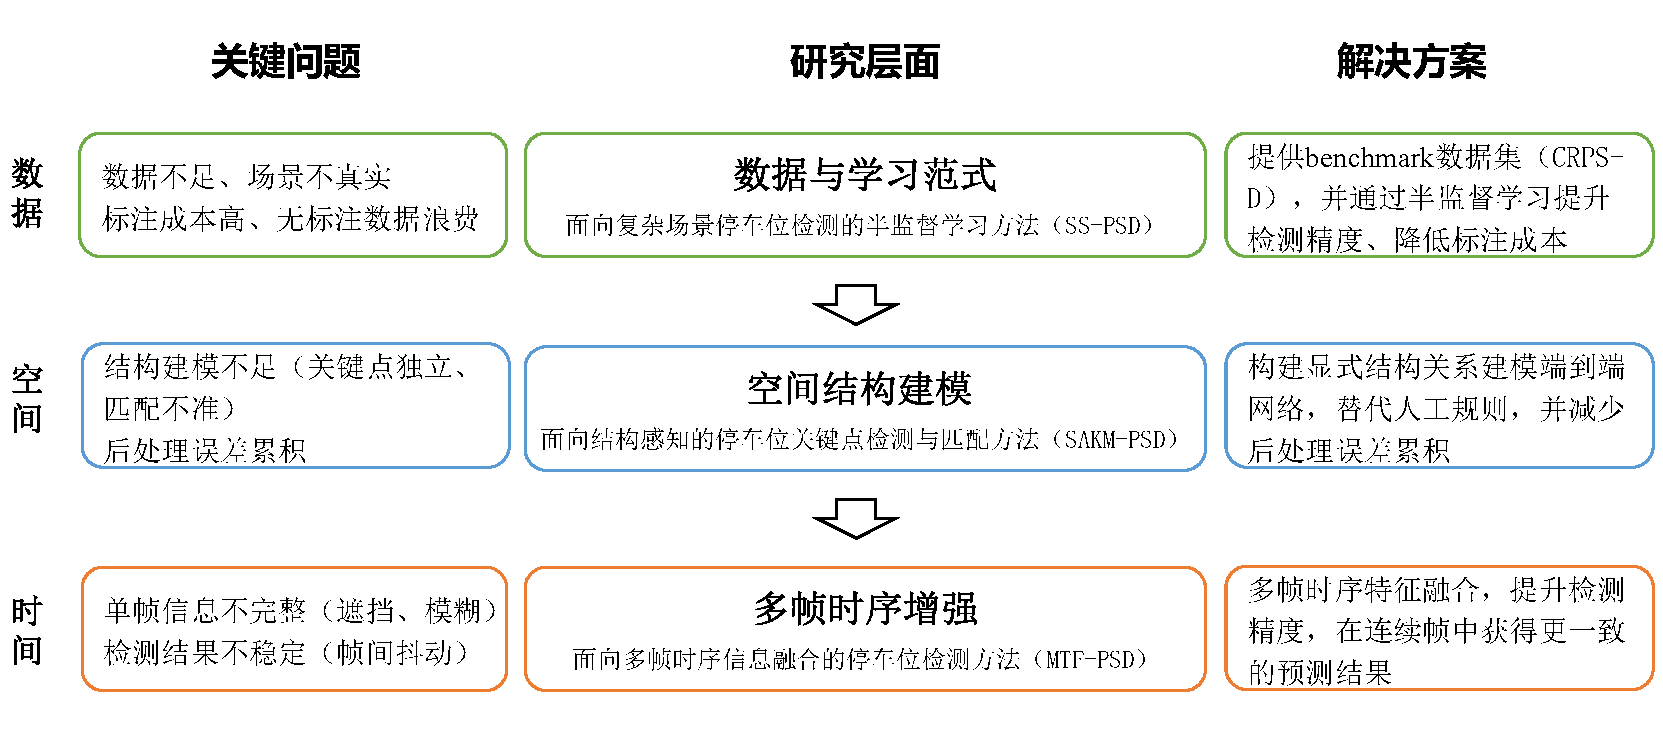
\includegraphics[width=1\linewidth]{figures/chp0/arch.pdf}
  \caption{论文研究内容  \\Figure~\ref{fig_arch}~Research content of the thesis}
  \label{fig_arch}
\end{figure}

\section{论文组织结构}

本章的整体结构安排如下：

第一章 绪论，本章介绍了研究背景与意义，分析了停车位检测在自动泊车系统中的关键作用，并总结了当前停车位检测技术面临的数据受限、空间结构建模不足以及时序信息利用不充分等挑战。并明确了本文的研究目标与主要贡献，概述了论文的整体组织结构。

第二章 相关理论，本章介绍了停车位检测领域通用框架、现有公开数据集、相关评价指标，以及半监督学习、注意力机制和时序建模的理论基础，为后续研究提供理论支撑。

第三章 面向复杂场景停车位检测的半监督学习方法，本章介绍了包含 35739 张图像的真实场景停车位检测数据集 CRPS-D，并对其特点进行定性与定量分析。同时提出了基于教师-学生架构的半监督学习框架 SS-PSD，通过置信度引导掩码一致性与自适应特征扰动机制挖掘无标签数据的空间先验，最后，通过多个实验验证了半监督学习在停车位检测中的有效性。

第四章 面向结构感知的停车位关键点检测与匹配方法，本章介绍了双分支检测框架 SAKM-PSD，包含结构感知 CutMix 策略、注意力引导插值模块与稀疏对匹配损失，实现了关键点定位与结构匹配的联合优化，增强模型对结构信息的感知能力与鲁棒性。最后，在ps2.0和 CRPS-D 数据集上验证了方法的有效性。

第五章 面向多帧时序信息融合的停车位检测方法，本章介绍了时序框架 MTF-PSD ，包含跨帧自注意力机制、动态结构感知时序融合模块及时序鲁棒增强策略，实现了时空联合感知的停车位检测。同时为了进一步评估方法的有效性，提出了PSTD 时序数据集，通过实验验证了多帧时序融合对检测性能的提升。最终，分析了 MTF-PSD 模型在实际车载平台上的推理效率。

第六章 总结与展望，本章总结了本文的主要工作与创新点，分析了所提出的方法在复杂场景下的优势与局限性，并展望了未来的研究方向，包括模型轻量化、多模态融合及端到端自动驾驶系统集成等。

